\subsection{Theorem}
\begin{namedframe}{Theorem}
	\begin{theorem}[``Star Trek'' Theorem]
		The central angle \alert{subtended} by any arc is twice any of the inscribed angles on that arc.

		This means that in the diagram, $\angle AOB = 2 \angle ACB$.
	\end{theorem}
	\pause
	\centering
	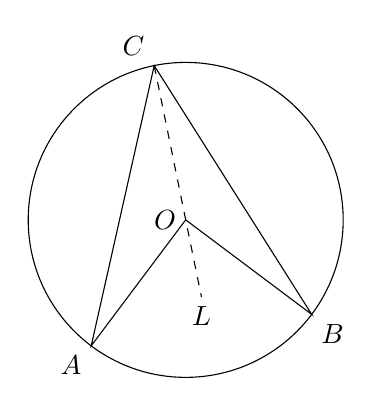
\begin{tikzpicture}[scale=0.4]
		\coordinate [label=left:$O$](O) at (0,0);
		\coordinate [label=below left:$A$](A) at (-3,-4);
		\coordinate [label=below right:$B$](B) at (4,-3);
		\coordinate [label=above left:$C$](C) at (-1,4.89897948557);
		\coordinate [label=below:$L$](L) at (0.5,-2.44948974278);

		\draw (O) circle (5);
		\draw (A) -- (O) -- (B) -- (C) -- cycle;
		\draw [dashed] (C) -- (L);
	\end{tikzpicture}
\end{namedframe}
